\documentclass[Orbiter User Manual.tex]{subfiles} 
\begin{document}

\section{Multi-functional display modes}
Multifunctional displays (or MFDs) are used in the cockpits of most military aircraft and modern airliners. The combine the function of a variety of traditional instruments in a compact format, and in combination with computerised avionics data processing they present the pilot with situation-dependent relevant data.\\
In spaceflight, providing the pilot with information appropriate to the current flight regime is even more critical, so for example the Space Shuttle made extensive use of MFD displays. Orbiter uses the MFD paradigm in a general and extendable way to provide flight data independent of vessel type (although vessel-specific MFD modes can be implemented by add-on developers).

\begin{figure}[H]
  \centering
  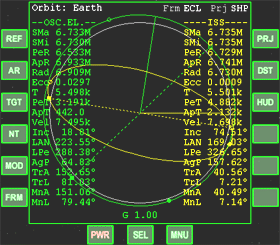
\includegraphics[width=0.5\hsize]{mfd_main.png}
\end{figure}

\noindent
The user interface of an MFD is essentially a computer display (e.g. an LED screen) and a set of input controls (usually push buttons arranged around the screen, or a separate keyboard). In Orbiter, all spacecraft MFDs work the same way, even if the specific layout varies. The picture shows the MFD representation for the generic cockpit view, which supports two MFD positions. 2D panel and virtual cockpit views may use a different number of MFD instruments.
In the centre of the MFD is the data display. The 12 buttons along the left and right edge are mode-dependent function buttons. Their labels may change according to the current operation modus of the instrument. The three buttons along the bottom edge are static and perform mode-independent system functions.\\
The MFDs can be operated either by left-clicking the buttons with the mouse, or via the keyboard. All MFD keyboard functions are \Shift-key combinations, where the left and right \Shift keys operate the left and right MFD, respectively. For instrument panels with more than two MFD displays, only two can be operated with the keyboard; the others are limited to mouse control.\\
\\
\textbf{Turning the MFD on and off}\\
The PWR button activates and deactivates the MFD display (keyboard shortcut: \Shift\keystroke{Esc}). In glass cockpit mode, turning off the MFD also hides the buttons (except the power button, so it can be turned on again).\\
\\
\textbf{Mode selection}\\
The SEL button activates the \textit{mode selection screen} (keyboard shortcut: \Ctrl\keystroke{F1}). Each MFD mode provides information for a different navigation or avionics situation (orbital parameters, surface parameters, docking and landing aids, etc.) The default modes are described below in this chapter. Many additional modes are available via 3$^{rd}$ party add-ons.\\
The mode selection screen shows the available modes in the display area, one mode next to each function button. To select a mode, simply click the corresponding button. For selection with the keyboard, press the \Ctrl key together with the mode selection key displayed in grey with each of the listed modes (for example, \Ctrl\keystroke{O} for Orbit mode).

\begin{figure}[H]
  \centering
  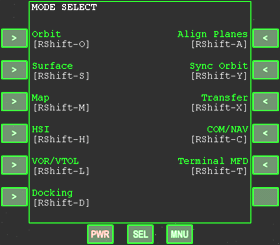
\includegraphics[width=0.5\hsize]{mfd_mode.png}
\end{figure}

\noindent
If there are more modes than can be displayed in a single page, pressing SEL (or \Ctrl\keystroke{F1}) repeatedly cycles through all mode pages. Pressing SEL on the last mode page returns to the previously selected MFD mode. Note that mode selection with keyboard shortcuts works from any of the mode selection pages, even if the requested mode is not displayed on the current page.\\
\\
\textbf{Function buttons}\\
The function of the buttons to the left and right of the display depends on the current MFD mode, and their labels change accordingly. Functions and user interface for the standard MFD modes are described below. For modes provided by 3$^{rd}$ party add-ons, consult the accompanying documentation. In some cases the buttons may act as switches, where each press executes a discrete operation. In other cases it may be necessary to press down a button continuously to adjust a parameter.

\begin{figure}[H]
  \centering
  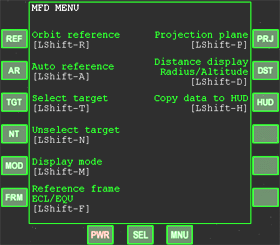
\includegraphics[width=0.5\hsize]{mfd_menu.png}
\end{figure}

\noindent
Function buttons for the two main MFD instruments can also be activated with \Ctrl-key combinations. On pressing the MNU button below the bottom edge of the screen (keyboard shortcut: \Ctrl\keystroke{`}) a short description of all function buttons for this mode is displayed, together with the keyboard shortcuts to activate them. Pressing MNU again, or pressing a function button, restores the display.\\
In glass cockpit view, and in most instrument panels in Orbiter, each MFD has 12 function buttons, but individual spacecraft can adopt a different layout in their panels. If an MFD mode assigns more function buttons than are physically present, pressing MNU repeatedly cycles through the available function pages.\\
\\
\textbf{Colour customisation}\\
The default colour schemes for MFD displays can be modified by editing the Config\textbackslash MFD\textbackslash default.cfg text file. Note that some add-on MFD Modes may define their own colour scheme which cannot be customised.


\subsection{NAV receiver/transmitter setup}
The \textit{COM/NAV setup} MFD mode provides an interface to the ship’s navigation radio receivers which feed data into the navigation instruments. It also allows to select the frequency of the ship’s long-range transponder which sends a signal identifying the vessel and its position. The mode is activated via the COM/NAV entry from the MFD mode selection page (shortcut: \Ctrl\keystroke{,} + \Ctrl\keystroke{.}).\\
\\
\textbf{Key options:}

%\begin{table}[H]
	%\centering
	\begin{longtable}{ |p{0.15\textwidth}|p{0.15\textwidth}|p{0.6\textwidth}| }
	\hline\rule{0pt}{2ex}
	\textbf{Button} & \textbf{Shortcut} & \textbf{Action}\\
	\hline\rule{0pt}{2ex}
	SL- & \Shift\keystroke{,} & Move selection up\\
	\hline\rule{0pt}{2ex}
	SL+ & \Shift\keystroke{.} & Move selection down\\
	\hline\rule{0pt}{2ex}
	<{}< & \Shift\keystroke{-} & Step frequency down 1 MHz\\
	\hline\rule{0pt}{2ex}
	>{}> & \Shift\keystroke{=} & Step frequency up 1 MHz\\
	\hline\rule{0pt}{2ex}
	< & \Shift\keystroke{[} & Step frequency down 0.05 MHz\\
	\hline\rule{0pt}{2ex}
	> & \Shift\keystroke{]} & Step frequency up 0.05 MHz\\
	\hline\rule{0pt}{2ex}
	SC< & \Shift\keystroke{Z} & Scan frequency downward\\
	\hline\rule{0pt}{2ex}
	SC> & \Shift\keystroke{X} & Scan frequency upward\\
	\hline
	\end{longtable}
%\end{table}

\noindent
\textbf{MFD control layout:}

\begin{figure}[H]
  \centering
  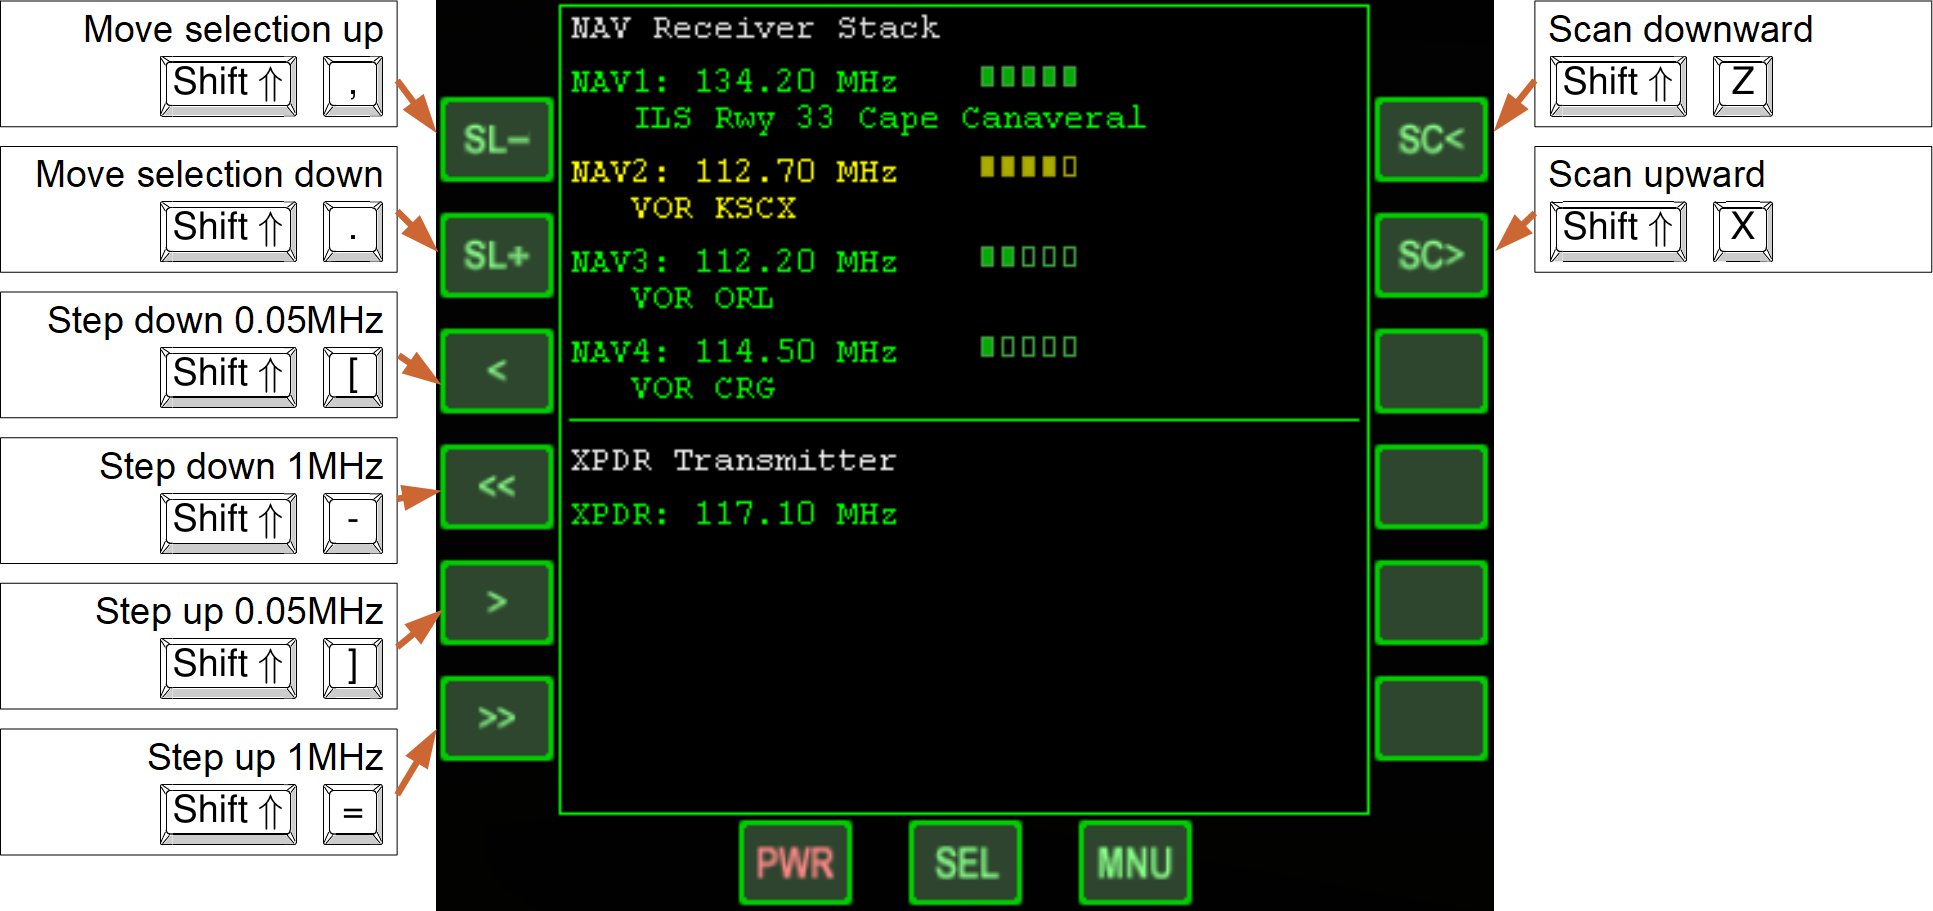
\includegraphics[width=0.99\hsize]{nav_input.png}
\end{figure}

\noindent
\textbf{MFD display components:}\\
The top part of the MFD display shows the NAV radio receiver stack. For each available receiver, the current frequency setting is shown, together with an identification of the received signal (if any) and a field strength indicator. The lower part of the display shows the transponder (XPDR) frequency.\\
The currently selected entry is highlighted in yellow. The selection can be moved up and down with the SL- (or \Shift\keystroke{,}) and SL+ (or \Shift\keystroke{.}) buttons.\\
The frequency of the selected receiver or transmitter can be tuned in steps of 1 MHz with \Shift\keystroke{-} and  \Shift\keystroke{=}, and in steps of 0.05 MHz with \Shift\keystroke{[} and \Shift\keystroke{]}, in the range from 108.00–140.00 MHz. You can sweep the frequency range down or up with \Shift\keystroke{Z} and \Shift\keystroke{X} until a signal is detected. If a compatible NAV transmitter is within range, the instrument displays information about the signal source and strength.

\begin{figure}[H]
  \centering
  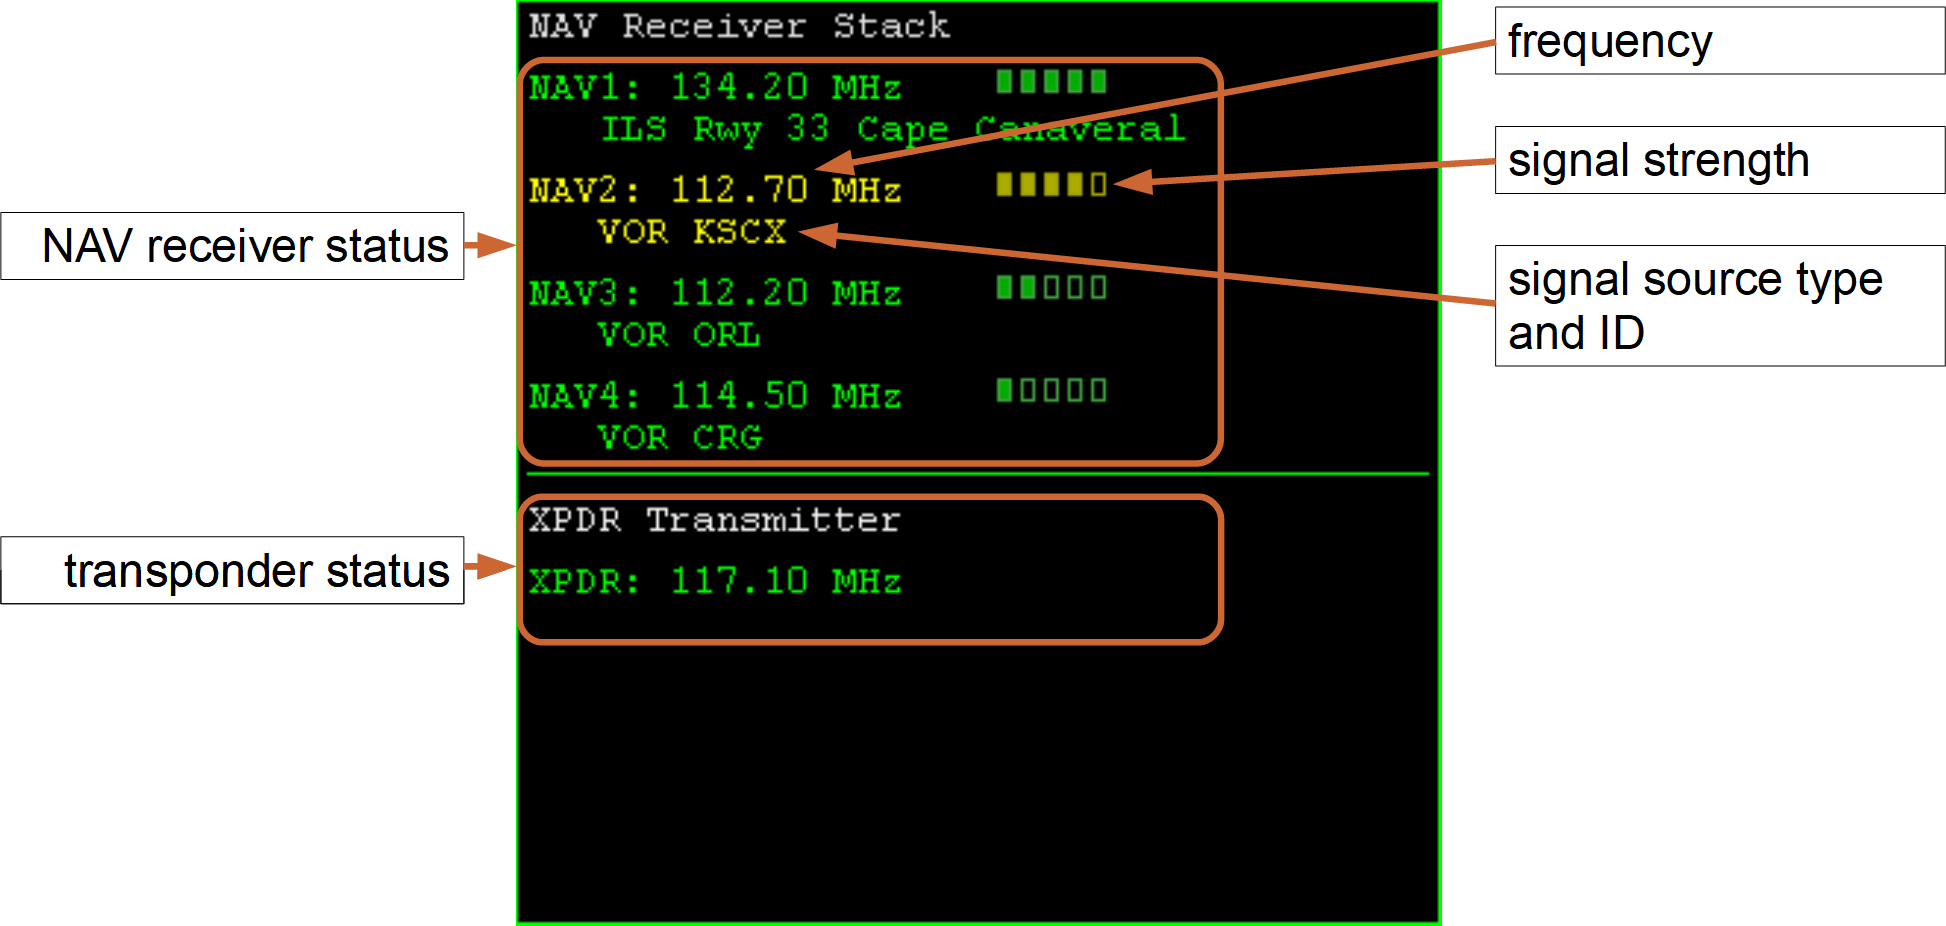
\includegraphics[width=0.99\hsize]{nav_layout.png}
\end{figure}

\noindent
In Orbiter, NAV transmitter types include VOR (VHF omnidirectional range), ILS (instrument landing system) for runway approaches and VTOL (vertical take-off and landing) pads, XPDR (vessel transponders) and IDS (instrument docking system). Each transmitter type provides information which can be fed to other MFD modes or avionics instrumentation to provide situational awareness to the pilot.\\
%TODO add section link
The \textit{Object info} (\Ctrl\keystroke{I}, see TODO) and \textit{Map} (\Ctrl\keystroke{M}, see TODO) windows are useful tools to obtain surface or vessel-based transmitter frequencies.

\begin{figure}[H]
  \centering
  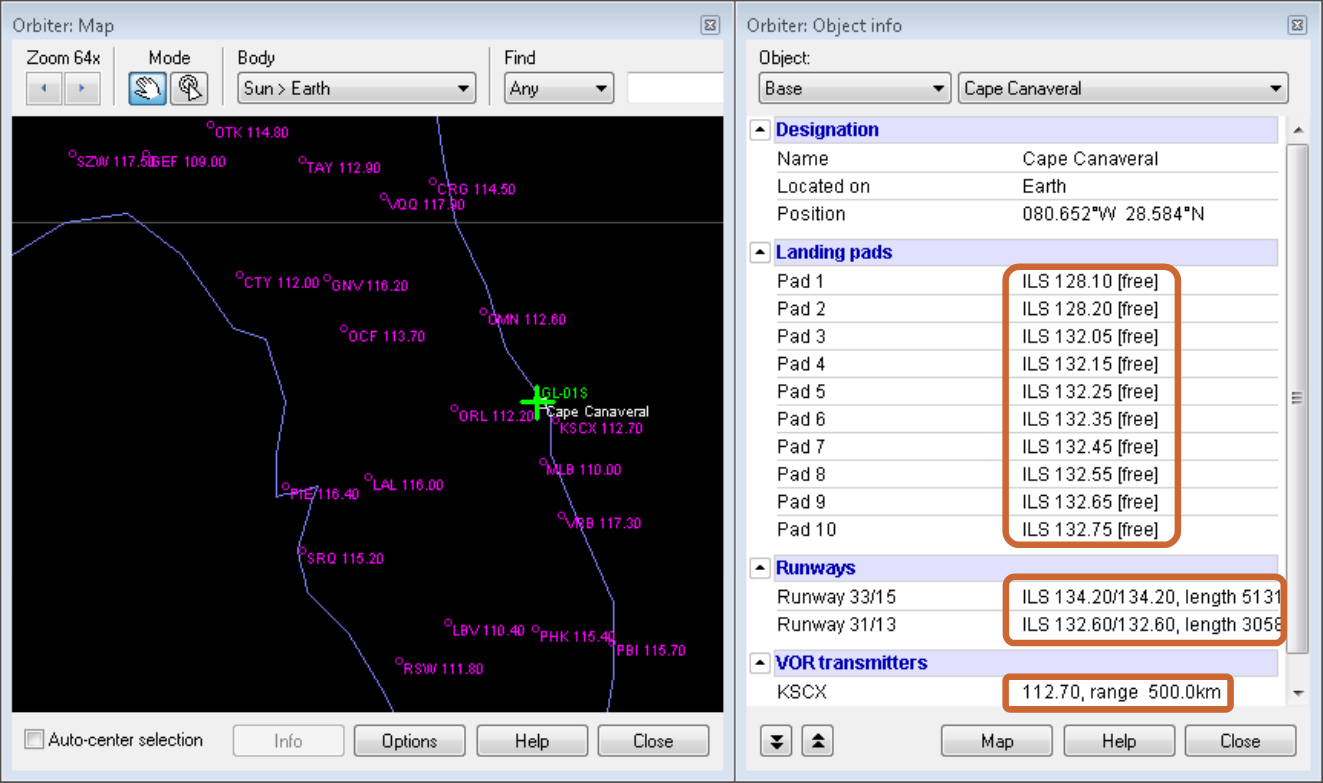
\includegraphics[width=0.75\hsize]{freq_map_info.png}
  \caption{Map window (left) and object info dialog (right) with NAV transmitter information}
\end{figure}

\noindent
The positions and frequencies of VOR stations in your vicinity can also be displayed directly in the simulation window via the VOR Markers option in the \textit{Visual helpers} dialog box (\Ctrl\keystroke{F9}).


\subsection{Surface}
% TODO

\subsection{Map}
% TODO

\subsection{VOR/VTOL}
% TODO

\subsection{Horizontal Situation Indicator}
% TODO

\subsection{Orbit}
% TODO

\subsection{Align Orbital Plane}
% TODO

\subsection{Synchronise orbit}
% TODO

\subsection{Docking}
% TODO

\subsection{RCS Attitude}
% TODO

\subsection{Transfer}
% TODO

\end{document}
